\documentclass[a4j]{jarticle}
%%  packages
\usepackage{amsmath,amssymb,ascmac}
\usepackage{bm}
\usepackage[dvipdfmx]{graphicx}
\usepackage{listings}
\usepackage[english]{babel}
\lstset{
 	%枠外に行った時の自動改行
 	breaklines = true,
 	%標準の書体
        basicstyle=\ttfamily\footnotesize,
        commentstyle=\footnotesize\bfseries,
        keywordstyle=\footnotesize\bfseries,
 	%枠 "t"は上に線を記載, "T"は上に二重線を記載
	%他オプション:leftline,topline,bottomline,lines,single,shadowbox
 	frame = single,
 	%frameまでの間隔(行番号とプログラムの間)
 	framesep = 5pt,
 	%行番号の位置
 	numbers = left,
	%行番号の間隔
 	stepnumber = 1,
	%タブの大きさ
 	tabsize = 4,
 	%キャプションの場所("tb"ならば上下両方に記載)
 	captionpos = t
}

%% math commands
\let \ds \displaystyle
\newcommand{\idiff}[3]{
  \frac{d^{#1} #2}{d #3^{#1}}
}
\newcommand{\diff}[3]{
  \frac{\mathrm{d}^{#1} #2}{\mathrm{d} #3^{#1}}
}
\newcommand{\pdiff}[3]{
  \frac{\partial^{#1} #2}{\partial #3^{#1}}
}



%% title configuration
\title{統計的機械学習 ID:04}
\author{05-161026 平出一郎}
\date{\today}


%% headings
\pagestyle{headings}
\markright{統計的機械学習 ID:04}




\begin{document}
%%  begin title page
\thispagestyle{empty}
\maketitle
\pagebreak


\section{}
$a=b=1,0.1,5$に対して$beta(x|a+4,b+1)$からのMH法をもちいたサンプリングにより$p(x \geq 0.5),p(x \geq 0.8)$を近似計算した。

提案分布$q(x|y)$には最小値$0$、最大値$1$、最頻値$y$の三角分布を用いた。
\lstinputlisting[caption=result]{result01.txt}
\lstinputlisting[caption=01.py,language=python]{01.py}


\section{}
$a=b=1,0.1,5$に対して$beta(x|a+4,b+1)$からのMH法をもちいたサンプリングにより$E[x|data],E[\pi \leq 0.1|data]$を近似計算した。

提案分布$q(x|y)$には最小値$0$、最大値$1$、最頻値$y$の三角分布を用いた。
\lstinputlisting[caption=result]{result02.txt}
\lstinputlisting[caption=02.py,language=python]{02.py}

\section{}
ギブスサンプリングを用いた2変数正規分布からのサンプリングを行い、分散共分散行列の固有ベクトルとその大きさとともに散布図を示す。

burn in期間としてサンプルの最初の2割ほどのサンプルは表示していない。


結果

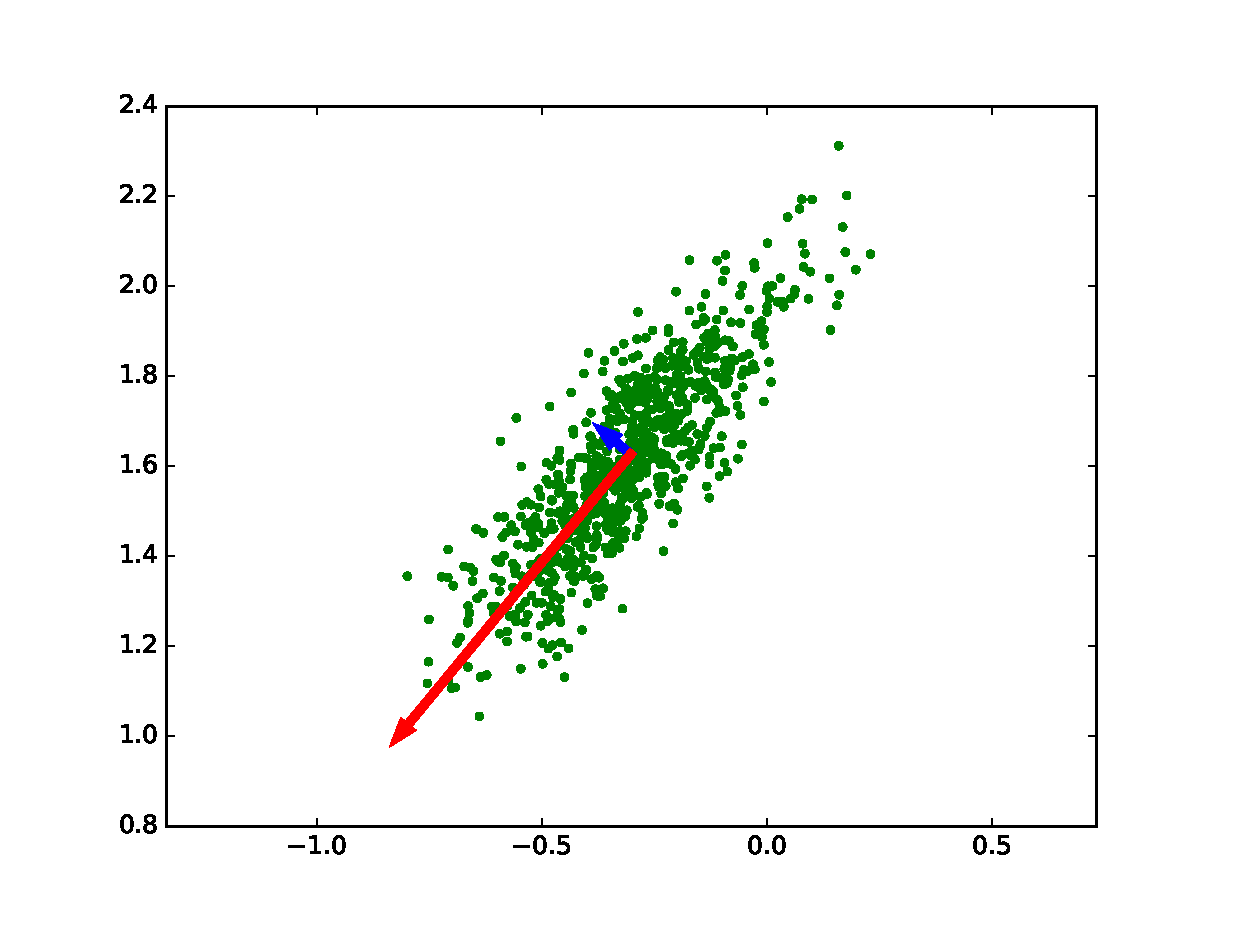
\includegraphics[width=10cm]{figure_1.eps}

\lstinputlisting[caption=03.py,language=python]{03.py}


\end{document}


